\documentclass[11pt]{article}

\usepackage[margin=0.85in]{geometry}
\usepackage[T1]{fontenc}
\usepackage{lmodern}
\usepackage{microtype}
\usepackage{amsmath,amssymb,amsthm}
\usepackage{enumitem}
\usepackage{titlesec}
\usepackage{graphicx}
\usepackage{tikz}
\usepackage{caption}

\setlength{\parindent}{0pt}
\setlength{\parskip}{5pt}
\setlist[enumerate]{leftmargin=1.45em,itemsep=3pt,topsep=4pt}
\setlist[itemize]{leftmargin=1.3em,itemsep=3pt,topsep=4pt}
\titlespacing*{\section}{0pt}{10pt}{3pt}
\titleformat{\section}{\large\bfseries}{}{0pt}{}
\captionsetup{font=small,labelfont=bf,skip=4pt}

\newtheorem{assumption}{Assumption}
\newtheorem{lemma}{Lemma}
\newtheorem{proposition}{Proposition}
\newtheorem{corollary}{Corollary}
\theoremstyle{definition}
\newtheorem{definition}{Definition}

\begin{document}

\begin{center}
{\LARGE\bfseries A Reproductive Closure for Housing-Market Economies}\par
\vspace{3pt}
{\large Theory note}\par
\vspace{3pt}
{\small August 11, 2026}
\end{center}

\vspace{-2pt}
This note develops, in general form, the population closure sketched in the
transition note: births must ultimately reproduce the population, and that
requirement---not migration or an outside option---pins the long-run housing
cost. The demographic condition selects the price; housing clearing then
selects the population. The note states the closure for a class of stationary
lifecycle economies and derives four results that do not depend on any
particular calibration. In words:

\begin{enumerate}
\item Housing can stabilize a population only if housing is a large enough
share of the marginal child's cost: the share must exceed the reproduction gap
(Section~4).
\item The slope of the reproduction schedule---how much fertility responds to
housing costs---is not identified by fertility levels and timing; it needs a
housing-cost response moment (Section~5).
\item Under this closure, housing supply cannot move the long-run price or
fertility; it only moves how many people live at the demographically pinned
price (Section~6).
\item The closed economy is the continuous limit of the open-economy
(inflow) closures, so nothing is knife-edge; the substantive question is
whether reproduction can reach replacement at all (Section~7).
\end{enumerate}

Section~8 gives the comparative statics and the honest transition language,
and Section~9 traces the closure's two schedules in the maintained
quantitative model.

\section*{1. Environment}

The note applies to any economy with the following five features. The
maintained quantitative model is one member of the class; the representative-family
model of the transition note is another.

\textbf{Agents.} Time is discrete. The economy is populated by overlapping
cohorts of households. A household enters adult life at a fixed age, lives at
most $J$ periods, and survives from one age to the next with exogenous
probabilities. Adult population is a mass $S$ of households; $g$ denotes the
composition of that population over individual states (age, income, wealth,
housing, children), normalized to integrate to one.

\textbf{Preferences.} Households value consumption, housing services, and
children. Each child living at home requires resources in two forms: goods and
space. The space requirement is what connects the price of housing to the cost
of a child; its exact form (a requirement per child, a discrete jump at the
first child, an equivalence scale) is left free.

\textbf{Endowments and technology.} Labor income per household is exogenous to
the economy's scale. Housing services are supplied along an aggregate schedule
$H^S(r)$, weakly increasing in the rental user cost $r$, in levels rather than
per household. A constant wedge $\rho$ ties the asset price to the user cost,
$P=r/\rho$; taxes inside $\rho$ are treated as parameters.

\textbf{Markets and institutions.} Households may rent or own; rental and owner
segments may carry size menus, borrowing limits, down payments, and
transaction costs. Any government budget is balanced by per-household taxes
and transfers. These institutions affect the results only through two
aggregate schedules defined below.

\textbf{Demography.} Children live at home, then mature. A maturing child
becomes a potential entrant household at conversion rate $c>0$ (children per
new household formed, inverted); a fraction $\ell\in[0,1)$ of born children
never mature into entrants because their household exits first. New households
enter at the fixed entry age.

Two assumptions make the closure well-defined.

\begin{assumption}[Scale invariance]\label{ass:scale}
Given $r$, the household problem and the per-household fiscal rules do not
depend on $S$. Aggregate scale affects households only through the housing
market.
\end{assumption}

Constant-returns production with an exogenous interest rate and a rebated tax
system deliver this. Under Assumption~\ref{ass:scale}, for each candidate $r$
there is a normalized stationary composition $g(r;\theta)$, where $\theta$
collects preference and policy parameters, and three per-household aggregates
are defined by integrating policies over $g$:

\begin{itemize}
\item $D(r;\theta)$: physical housing demand per household;
\item $\beta_f(r;\theta)$: births per household per period;
\item $B(r;\theta)=c\,[1-\ell(r;\theta)]\,\beta_f(r;\theta)$: mature entrant
households generated per incumbent household per period.
\end{itemize}

\begin{assumption}[Exogenous survival]\label{ass:surv}
Survival probabilities depend on age only, and entry occurs at a single age.
\end{assumption}

\begin{lemma}[The replacement requirement is a demographic constant]\label{lem:E}
Under Assumption~\ref{ass:surv}, the inflow of entrant households required to
reproduce one unit of the stationary composition is
$E=1/\sum_{j=0}^{J-1} s_j$, where $s_j$ is the probability of surviving to age
$j$. It does not depend on $r$, $\theta$, or policy.
\end{lemma}

The age distribution of a stationary population is pinned by survival alone,
so the entering cohort's share of the population---equivalently, deaths per
household per period---is a number, not a schedule. The closure below is
therefore one equation in one unknown.

It is convenient to express reproduction in child units. Since a household
lives $1/E$ periods on average, lifetime births per household are
$\nu(r;\theta)=\beta_f(r;\theta)/E$, and the condition $B=E$ is equivalent to
\begin{equation}
\nu(r;\theta)=\bar n^{*}\equiv\frac{1}{c\,(1-\ell)} .
\label{eq:replacement_units}
\end{equation}
The right-hand side is replacement in the model's own units: the births a
household must produce so that, after conversion into new households and the
loss of children whose household exits first, it exactly replaces itself.

\section*{2. The closure family}

Every stationary version of the economy must state where entrant households
come from. The general balance condition is
\begin{equation}
S\,E \;=\; \bar R\,S\,B(r;\theta)\;+\;\bar M ,
\label{eq:family}
\end{equation}
with retention $\bar R\in(0,1]$ of locally born entrants and an outside inflow
$\bar M\ge0$. The left side is the entrant flow a population of size $S$
requires; the right side is the flow it receives. Three known cases are the
value-based entry probability (which makes $\bar R$ and the split of
$\bar M$ respond to $r$ through an outside option), the fixed quota
($\bar R,\bar M$ fixed), and the closed economy ($\bar R=1$, $\bar M=0$).

The cases differ in which equation determines which unknown. With $\bar M>0$,
condition \eqref{eq:family} determines $S$ given $r$, and housing clearing
determines $r$: demography and the housing market are solved jointly. With
$\bar M=0$ the condition becomes scale-free---$S$ multiplies both sides---so
it can no longer determine the population. It becomes a restriction on the
price:
\begin{equation}
B(r^{*};\theta)=E .
\label{eq:reproduction}
\end{equation}
Housing clearing, now free, determines the population. This reallocation of
equations to unknowns is the entire content of the closure.

\begin{definition}[Reproductive stationary equilibrium]\label{def:rse}
A reproductive stationary equilibrium is a user cost $r^{*}$, a normalized
composition $g^{*}$, and an adult population $S^{*}$ such that:
(i) households optimize at $r^{*}$ and $g^{*}=g(r^{*};\theta)$ is the implied
stationary composition; (ii) reproduction is at replacement,
$B(r^{*};\theta)=E$; and (iii) the housing market clears in levels,
$S^{*}D(r^{*};\theta)=H^S(r^{*})$.
\end{definition}

\begin{proposition}[Existence and uniqueness]\label{prop:exist}
Suppose $B(\cdot;\theta)$ is continuous on an interval $[r_\ell,r_h]$ with
$B(r_\ell;\theta)>E>B(r_h;\theta)$. Then an equilibrium exists. If in addition
$B$ is strictly decreasing where it crosses $E$, the reproductive price
$r^{*}$ is unique, and $S^{*}=H^S(r^{*})/D(r^{*};\theta)$ is unique and
positive whenever $H^S(r^{*})>0$ and $D(r^{*};\theta)>0$.
\end{proposition}

The proof is the intermediate value theorem plus monotonicity; the economics
is in the premises. Continuity holds when birth and housing choices are
smoothed by taste shocks and the income process mixes; purely deterministic
discrete choices can put steps into $B$. The boundary condition---reproduction
above replacement when housing is cheap, below when it is expensive---is the
substantive requirement, and Section~4 restates it in observables. Nothing
guarantees it: it is where a proposed closure of this kind succeeds or fails.

\section*{3. Reading the child decision into the schedule}

The schedule $B(r;\theta)$ aggregates the household birth margin, so the
comparative statics of the closure inherit their sign from the household
problem. At the household level the full price of a child is
\begin{equation}
p_c(r)\;=\;\chi\;+\;m(r),
\label{eq:childprice}
\end{equation}
where $\chi$ collects the goods components (consumption requirements and any
goods-denominated frictions) and $m(r)$ collects the housing components: the
child's space requirement valued at the household's effective marginal cost of
space. For an unconstrained renter that cost is $r$ itself; for a household at
a rental size limit or a down-payment margin it is $r$ plus the goods value of
the binding constraint. The important property of $m$ is that its constituents
scale with prices: rent, maintenance, the down payment $(1-\phi)P h$, and
proportional transaction costs are all linear in $r$ or in $P=r/\rho$, so
$m(0)=0$ and $m$ is increasing.\footnote{A rental size cap does not itself
vanish as $r\to0$, but the ownership route around it does: the down payment on
any house goes to zero with the price, so the cap's wedge is eventually
price-eliminable. Genuinely price-proof components---fixed goods costs of
moving or originating a mortgage---belong in $\chi$.}

Two households with the same preferences but different constraint positions
face different $m(r)$, which is why $B$ is an aggregate over $g$ and not a
representative demand curve. The representative-family demand of the
transition note, $n=\beta/(b+ap)$, is the special case of a single
unconstrained household with linear $m$.

\section*{4. When can housing stabilize the population?}

The boundary premise of Proposition~\ref{prop:exist} asks whether cheap
housing can push reproduction above replacement. Because housing prices can
only fall to zero, the housing channel is a bounded stabilizer: it can remove
at most the housing component of the child's price. This gives an existence
condition in observables.

Let $\nu(r)=F\!\left(p_c(r);\theta\right)$ with $F$ decreasing in the child
price, let $r_0$ denote the current housing cost, and define two statistics at
$r_0$: the \emph{reproduction gap}
\[
\gamma\;\equiv\;1-\frac{\nu(r_0)}{\bar n^{*}},
\]
the shortfall of lifetime births from replacement, and the \emph{housing share
of the marginal child's cost}
\[
s_H\;\equiv\;\frac{m(r_0)}{\chi+m(r_0)} .
\]

\begin{proposition}[Stabilization condition]\label{prop:stab}
A reproductive price $r^{*}\in(0,r_0]$ exists if and only if fertility at the
housing-free child price reaches replacement, $F(\chi;\theta)\ge\bar n^{*}$.
In the benchmark case $F(p)=\beta/p$, this holds if and only if
\begin{equation}
s_H\;\ge\;\gamma .
\label{eq:gapshare}
\end{equation}
\end{proposition}

\begin{proof}
$p_c$ is continuous and increasing with $p_c(0)=\chi$, so
$\nu(0)=F(\chi;\theta)$ is the supremum of $\nu$ on $[0,r_0]$ and the
intermediate value theorem applies. In the benchmark,
$\nu(0)/\nu(r_0)=p_c(r_0)/\chi=1/(1-s_H)$, and
$\nu(0)\ge\bar n^{*}$ rearranges to $s_H\ge1-\nu(r_0)/\bar n^{*}=\gamma$.
\end{proof}

Housing can restore replacement only if the share of the marginal child's cost
that prices can remove is at least the current reproduction gap. Both sides
are measurable without solving a model: the gap from vital statistics and
household-formation rates, the share from child-cost accounting or---because
in the benchmark the local elasticity of fertility with respect to the housing
cost \emph{equals} $s_H$---from quasi-experimental estimates of the fertility
response to housing costs. The condition also says where to look when a
quantitative economy fails it: either children's costs load mostly on goods,
or the model's fertility margin is too price-insensitive. The next section
shows the second failure can be an artifact of identification rather than a
finding.

Constraint wedges sharpen rather than weaken the condition's content. For a
household at a rental cap or a collateral margin, $m$ includes the wedge, so
$s_H$ is \emph{larger} exactly for the households at the birth margin---the
access-constraint mechanism raises the stabilizer's strength. What bounds the
stabilizer is the goods component $\chi$ and any friction denominated in goods
rather than in house value.

\section*{5. What disciplines the slope}

Existence, uniqueness, and every comparative static below run through the
slope of $B$ in $r$. In discrete-choice implementations of fertility, that
slope is not identified by the stationary fertility facts a calibration
usually targets.

Consider the simplest case: one lifetime birth decision, taken when the
consumption-equivalent surplus of a child is $d=b_s-p_c(r)$, with $b_s$ the
non-housing child surplus, smoothed by a taste shock of scale $\sigma$ in
goods units, so that $\nu=\Lambda(d/\sigma)$ for a logistic $\Lambda$. Then
\begin{equation}
-\frac{\partial\ln\nu}{\partial\ln r}
\;=\;
s_H\;\times\;\underbrace{(1-\nu)\,\frac{p_c}{\sigma}}_{\text{response factor}} .
\label{eq:attenuation}
\end{equation}
The elasticity is the cost share times a response factor that the noise scale
drives anywhere in $(0,\infty)$. Matching the \emph{level} of fertility pins
$d/\sigma$, and matching timing and dispersion constrains the distribution of
$d/\sigma$ across households---but $p_c/\sigma$ remains free: doubling both
the surplus and the noise leaves every stationary fertility fact unchanged and
halves the price response. Two economies with identical fertility levels,
timing, and childlessness can therefore carry arbitrarily different
reproduction schedules $B(r)$.

The implication is an identification requirement, not a modeling choice: a
quantitative implementation of the closure---or of any exercise whose answer
runs through the fertility--housing-cost margin---needs at least one moment
that measures a fertility response to a housing-cost change (a
quasi-experimental price or credit shock), on top of the stationary fertility
facts. Absent such a moment, the slope of the reproduction schedule, and with
it $r^{*}$ and all long-run policy responses, are conventions of the noise
scale.

\section*{6. What the closure implies in the long run}

Two invariance results follow directly from the equilibrium structure, and
they reorganize what a policy exercise can claim.

\begin{proposition}[Supply neutrality]\label{prop:supply}
Any change to the supply schedule $H^S(\cdot)$ alone leaves $r^{*}$,
$g^{*}$, and every per-household statistic unchanged, and moves the
population proportionally: $S^{*}=H^S(r^{*})/D(r^{*};\theta)$.
\end{proposition}

The reproductive condition \eqref{eq:reproduction} contains no supply objects,
so supply cannot move the long-run price. The contrast with open closures is
sharp: with $\bar M>0$, supply expansion lowers the equilibrium user cost and
raises reproduction; under the closed closure the same expansion changes how
many households live at the demographically pinned price. Whether ``build more
housing'' is an affordability policy or a population policy in the long run is
decided by the demographic closure, not by the housing block. This is the
Malthusian structure inverted into housing: the reproductive margin pins the
price of the scarce factor, and supply pins the scale of the population, just
as the subsistence margin once pinned the wage.

\begin{proposition}[Reproduction is not a long-run outcome variable]\label{prop:invariance}
Across reproductive stationary equilibria---across policies, preferences, or
supply regimes---lifetime births per household equal $\bar n^{*}$ and the
stock of children at home per household equals the birth flow times mean years
at home, both invariant up to the (second-order) dependence of the loss rate
$\ell$ on birth timing.
\end{proposition}

Long-run fertility is at replacement in every such equilibrium by
construction. What policy moves is the price at which replacement is
achieved, the population carried at that price, the timing of births, and the
composition of who has children. Total births move one-for-one with $S^{*}$.
A policy exercise under this closure should therefore report $(r^{*},
S^{*})$, timing, and composition---and should not describe a long-run TFR
response, which is zero by construction. The interesting statement runs the
other way: policies that make children cheaper raise the housing cost the
economy can sustain at replacement, and with it the population.

\section*{7. The open economy as a perturbation}

The closed closure is not an isolated construction; it is the continuous limit
of the family \eqref{eq:family}.

\begin{proposition}[Limit of the quota closure]\label{prop:limit}
Fix $\bar R=1$ and let $\bar M\downarrow0$. If $B(\cdot;\theta)$ crosses $E$
at $r^{*}$ from above and the clearing locus $S_c(r)=H^S(r)/D(r;\theta)$ is
increasing, then the open-economy equilibrium $(r_{\bar M},S_{\bar M})$
converges to the reproductive equilibrium $(r^{*},S^{*})$. If instead
$B(r;\theta)<E$ everywhere, then $S_{\bar M}\to0$: the closed limit of a
permanently sub-replacement economy is an empty one.
\end{proposition}

\begin{proof}[Proof sketch]
With $\bar M>0$ the demographic locus is $S_d(r)=\bar M/[E-B(r;\theta)]$,
defined and decreasing in $r$ where $B<E$, and diverging as $r\downarrow
r^{*}$. Its intersection with the increasing locus $S_c$ is unique. As
$\bar M\downarrow0$, $S_d$ falls pointwise for every $r$ bounded away from
$r^{*}$, so the intersection's price converges to $r^{*}$ and its population
to $S_c(r^{*})=S^{*}$. Without a crossing, $S_d\to0$ pointwise and the
intersection collapses to the origin.
\end{proof}

Three readings. First, there is no knife edge: an economy with a small outside
inflow behaves like the closed economy, deviating continuously in $\bar M$.
Second, the dichotomy in the proposition is the empirical sorting question:
an economy whose reproduction schedule never reaches replacement is
\emph{sustained} by its inflow, and modeling it closed forecasts extinction,
not a steady state. Third, the proposition locates the two closures on one
figure, which is how the paper should draw it (Figure~\ref{fig:loci}).

\begin{figure}[ht!]
\centering
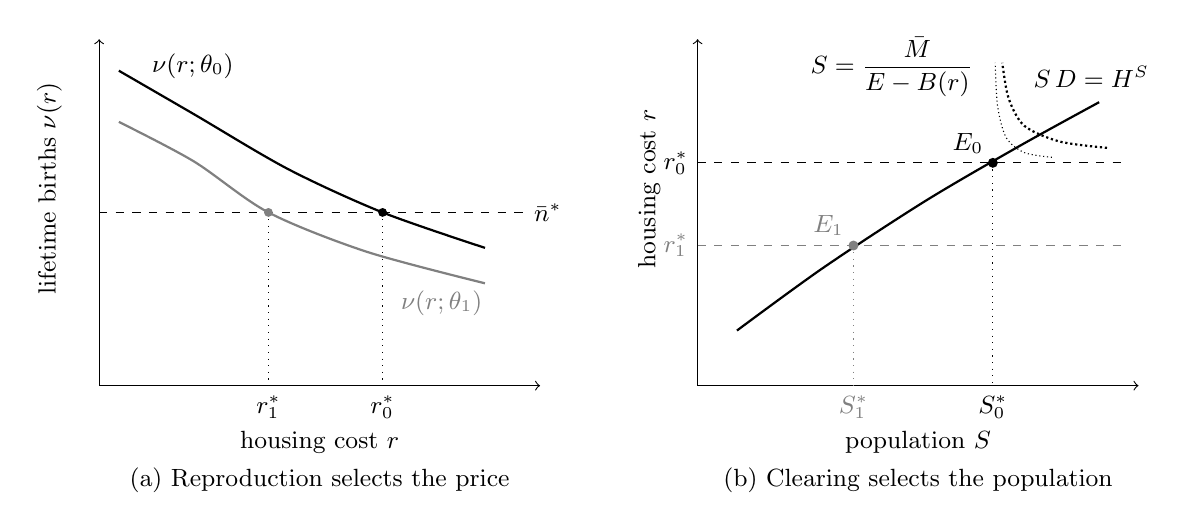
\begin{tikzpicture}[scale=1.0]
%----------------- Panel (a): reproduction selects the price -----------------
\begin{scope}[xshift=0cm]
\draw[->] (0,0) -- (5.6,0);
\draw[->] (0,0) -- (0,4.4) node[rotate=90, anchor=south, xshift=-1.9cm, yshift=0.35cm] {\small lifetime births $\nu(r)$};
\node at (2.8,-0.72) {\small housing cost $r$};
% replacement line
\draw[dashed] (0,2.2) -- (5.4,2.2);
\node[right] at (5.4,2.2) {\small $\bar n^{*}$};
% old schedule
\draw[thick, smooth] plot coordinates {(0.25,4.0) (1.2,3.45) (2.4,2.75) (3.6,2.2) (4.9,1.75)};
\node[above right] at (0.55,3.78) {\small $\nu(r;\theta_0)$};
% new schedule
\draw[thick, smooth, gray] plot coordinates {(0.25,3.35) (1.2,2.85) (2.15,2.2) (3.4,1.7) (4.9,1.3)};
\node[gray] at (4.35,1.05) {\small $\nu(r;\theta_1)$};
% roots
\draw[dotted] (3.6,2.2) -- (3.6,0) node[below] {\small $r_0^{*}$};
\draw[dotted] (2.15,2.2) -- (2.15,0) node[below] {\small $r_1^{*}$};
\fill (3.6,2.2) circle (1.6pt);
\fill[gray] (2.15,2.2) circle (1.6pt);
\node at (2.8,-1.2) {\small (a) Reproduction selects the price};
\end{scope}
%----------------- Panel (b): clearing selects the population ----------------
\begin{scope}[xshift=7.6cm]
\draw[->] (0,0) -- (5.6,0);
\draw[->] (0,0) -- (0,4.4) node[rotate=90, anchor=south, xshift=-1.9cm, yshift=0.35cm] {\small housing cost $r$};
\node at (2.8,-0.72) {\small population $S$};
% clearing locus (theta0)
\draw[thick, smooth] plot coordinates {(0.5,0.7) (1.6,1.5) (2.9,2.35) (4.1,3.05) (5.1,3.6)};
\node[above] at (5.0,3.66) {\small $S\,D=H^S$};
% reproductive prices
\draw[dashed] (0,2.83) -- (5.4,2.83);
\node[left] at (0,2.83) {\small $r_0^{*}$};
\draw[dashed, gray] (0,1.78) -- (5.4,1.78);
\node[left, gray] at (0,1.78) {\small $r_1^{*}$};
% equilibria on the clearing locus
\fill (3.75,2.83) circle (1.8pt) node[above left] {\small $E_0$};
\fill[gray] (1.98,1.78) circle (1.8pt) node[above left, gray] {\small $E_1$};
\draw[dotted] (3.75,2.83) -- (3.75,0) node[below] {\small $S_0^{*}$};
\draw[dotted, gray] (1.98,1.78) -- (1.98,0) node[below, gray] {\small $S_1^{*}$};
% open-economy demographic locus, two inflow levels, converging to E0
\draw[densely dotted, thick, smooth] plot coordinates {(5.2,3.02) (4.6,3.10) (4.15,3.30) (3.95,3.65) (3.87,4.1)};
\draw[densely dotted, smooth] plot coordinates {(4.5,2.90) (4.15,2.96) (3.92,3.15) (3.81,3.55) (3.78,4.1)};
\node[left] at (3.62,4.05) {\small $S=\dfrac{\bar M}{E-B(r)}$};
\node at (2.8,-1.2) {\small (b) Clearing selects the population};
\end{scope}
\end{tikzpicture}
\caption{The reproductive closure and its open-economy perturbation
(schematic). Panel (a): lifetime births per household against the housing
cost; the replacement line $\bar n^{*}$ selects the reproductive price. A
weaker desire for children shifts the schedule down and the price falls from
$r_0^{*}$ to $r_1^{*}$. Panel (b): the housing-market clearing locus in the
population--price plane; the reproductive prices select $S_0^{*}$ and
$S_1^{*}$. The dotted curves are the open-economy demographic locus
$S=\bar M/[E-B(r)]$ for two inflow levels: as $\bar M\downarrow0$ its
intersection with the clearing locus slides into the reproductive equilibrium
(Proposition~\ref{prop:limit}). For clarity the clearing locus is drawn for
one parameterization; a preference change also shifts it, and the
population comparison in Section~8 accounts for that.}
\label{fig:loci}
\end{figure}

\section*{8. Comparative statics and transitions}

\textbf{Prices.} At a regular root, implicit differentiation of
\eqref{eq:reproduction} gives
\[
\frac{dr^{*}}{d\theta}
=-\frac{\partial B/\partial\theta}{\partial B/\partial r},
\]
so any parameter that shifts reproduction down at given prices---a weaker
desire for children, a higher goods cost of children---lowers the long-run
housing cost, provided $B$ is locally decreasing in $r$. Policies enter the
same way: a down-payment grant or a property-tax change (which moves the wedge
$\rho$ and hence the asset price at a given user cost) shifts $B(\cdot;\theta)$
and moves $r^{*}$; a pure supply policy does not (Proposition~\ref{prop:supply}).

\textbf{Population.} Log-differentiating $S^{*}=H^S(r^{*})/D(r^{*};\theta)$,
\begin{equation}
d\ln S^{*}
=\bigl[\eta_S(r^{*})+\eta_D(r^{*})\bigr]\,d\ln r^{*}
\;-\;\left.\frac{\partial\ln D}{\partial\theta}\right|_{r}\,d\theta ,
\label{eq:dS}
\end{equation}
with $\eta_S\ge0$ the supply elasticity and $\eta_D=-\partial\ln D/\partial\ln
r\ge0$ the demand response. The first term is the toy model's channel: a lower
reproductive price supports fewer households because supply shrinks and each
household uses more space. The second is the composition term the
representative-family model cannot see. Proposition~\ref{prop:invariance}
bounds it: across reproductive steady states the child-driven component of
demand is pinned, so the composition term works only through timing, the
distribution of children across households, and tenure. When it is small, a
weaker desire for children lowers both the long-run housing cost and the
long-run population---the transition note's conclusion, now with its exact
conditions attached.

\textbf{Transitions.} Everything above compares stationary states. The natural
dynamic reading uses the separation of time scales: housing prices clear
within a period, while the demographic state adjusts over generations. In the
one-state (adiabatic) reduction, population drifts by the reproduction gap,
$\dot S_t/S_t\propto B(r_t)-E$, with $r_t$ clearing the housing market at
$S_t$; convergence to the new steady state is monotone under the same slope
conditions as Proposition~\ref{prop:exist}. The full model's transition adds
the age composition and, with durable housing, the stock as state variables;
cohort echoes can make the exact path non-monotone. The honest scope is
therefore: endpoints and their comparative statics are equilibrium objects;
the arrow between them is intuition until a calendar-time path is computed.

\section*{9. The two schedules in the quantitative model}

Everything above reads off two curves, and both are cheap to compute: a
fixed-price solve of the stationary model (one household solution, one
distribution pass, no equilibrium loop) delivers $B$, $E$, and $D$ at that
price. Figure~\ref{fig:trace} traces them in the maintained quantitative
model at one certified parameterization, holding the benchmark fiscal policy
fixed, on 37 prices from 3 to 310 percent of the benchmark.\footnote{Smoke
grade: a coarse wealth grid, so shapes and demographic ratios are reliable
(the benchmark reproduction ratio matches the production solution to four
digits) while levels carry about a one percent error. Full provenance and the
data are in \texttt{output/model/reproductive\_closure\_trace\_20260811/}.}

\begin{figure}[ht!]
\centering
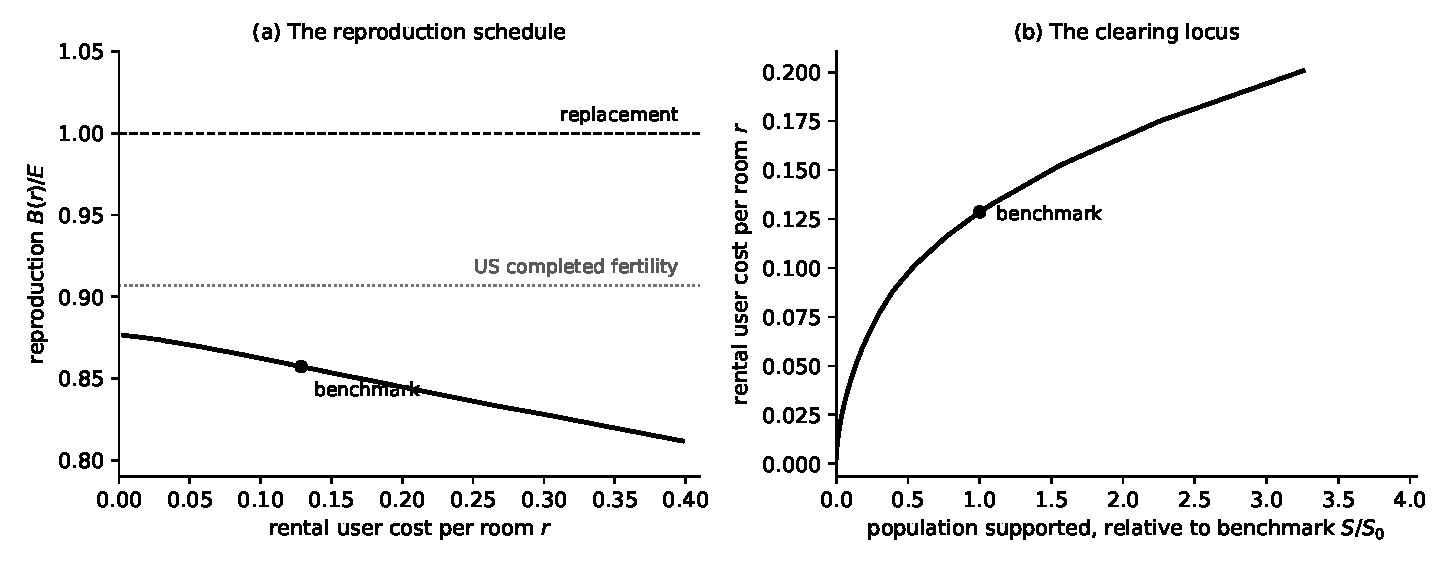
\includegraphics[width=0.99\textwidth]{../output/model/reproductive_closure_trace_20260811/reproduction_and_clearing_loci.pdf}
\caption{The closure's two schedules, computed from the quantitative model at
fixed prices (diagnostic grade). Panel (a): mature entrant households per
incumbent household, relative to the replacement requirement, against the
rental user cost. The replacement requirement $E=0.0617$ is identical at every
point, as Lemma~\ref{lem:E} says. Panel (b): the population supported by
housing clearing at each price, relative to the benchmark.}
\label{fig:trace}
\end{figure}

The trace verifies the theory's maintained slopes: the reproduction schedule
falls in the price everywhere, and the clearing locus rises. It also answers
the existence question for this parameterization, and the answer organizes the
rest of the agenda. The schedule is nearly flat---reproduction rises only from
$0.857$ at the benchmark to a ceiling of $0.876$ as housing becomes free---so
it never reaches the replacement line: at this parameterization the economy
has no closed reproductive steady state and is sustained by its entrant inflow,
the second branch of Proposition~\ref{prop:limit}. Read through
Proposition~\ref{prop:stab}, the model currently implies an effective housing
share of the marginal child's cost of about two percent, against a
reproduction gap of fourteen percent.

That implied share is far below child-cost accounting, and Section~5 says why
this is the right place to be suspicious rather than conclusive: the schedule's
slope is governed by the fertility choice-noise scale, which the stationary
fertility targets do not discipline. The trace therefore sharpens the agenda
to two measurements, in order of leverage:

\begin{enumerate}
\item \textbf{Discipline the slope.} Bring one quasi-experimental
fertility-response-to-housing-cost moment into the identification set. It
decides whether panel (a) is genuinely flat---housing cannot stabilize this
population---or an artifact of the noise scale.
\item \textbf{Measure the demographic constants.} The conversion $c$ (headship
of newly formed households) and the loss rate $\ell$ define replacement in
\eqref{eq:replacement_units} and hence where the replacement line sits.
Current vital statistics---completed fertility below household-unit
replacement, positive net entrant inflow---place the observed economy in the
open region either way, which is what makes the closed closure the benchmark
and the inflow the natural perturbation, rather than the reverse.
\end{enumerate}

\end{document}
